\documentclass[a4paper]{scrartcl}
%\documentclass[a4paper]{report}

% Uncomment to optimize for double-sided printing.
% \KOMAoptions{twoside}

% Set binding correction manually, if known.
% \KOMAoptions{BCOR=2cm}

% Localization options
\usepackage[english]{babel}
\usepackage[T1]{fontenc}
\usepackage[utf8]{inputenc}

% Enhanced verbatim sections. We're mainly interested in
% \verbatiminput though.
\usepackage{verbatim}

% PDF-compatible landscape mode.
% Makes PDF viewers show the page rotated by 90°.
\usepackage{pdflscape}

% Advanced tables
\usepackage{tabu}
\usepackage{longtable}

% Fancy tablerules
\usepackage{booktabs}

% Graphics
\usepackage{graphicx}

% Current time
\usepackage[useregional=numeric]{datetime2}

% Float barriers.
% Automatically add a FloatBarrier to each \section
\usepackage[section]{placeins}

% Custom header and footer
% \usepackage{fancyhdr}
% \setlength{\headheight}{15.2pt}
% \pagestyle{fancyplain}

\usepackage{geometry}
\usepackage{layout}

\usepackage{subcaption}

% Math tools
\usepackage{mathtools}
% Math symbols
\usepackage{amsmath,amsfonts,amssymb}

% \fancyhf{}
% % Chapter header on non-plain pages only.
% \lhead{\fancyplain{} {\leftmark}}
% % Footer must contain print date. Ugly, but IPA requirement.
% \lfoot{\printdate}
% % Print date left and page count right was the thing which looked the
% % most balanced.
% \rfoot{\thepage}
% 
% Source code & highlighting
\usepackage{listings}

\DeclarePairedDelimiter\floor{\lfloor}{\rfloor}
\DeclarePairedDelimiter\abs{\lvert}{\rvert}

% Convenience commands
\newcommand{\mailsubject}{2409 - Datenstrukturen und Algorithmen - Series 6}
\newcommand{\maillink}[1]{\href{mailto:#1?subject=\mailsubject}
                               {#1}}

% Should use this command wherever the print date is mentioned.
\newcommand{\printdate}{\today}

\subject{2409 - Datenstrukturen und Algorithmen}
\title{Series 6}

\author{Michael Senn - 16-126-880}

\date{}

% Needs to be the last command in the preamble, for one reason or
% another. 
\usepackage{hyperref}


\begin{document}
\maketitle

\section{Manual hash functions}

Using the given hash function

\[
	h(k) = \floor*{m * \left( k * \frac{\left( \sqrt(5) - 1 \right)}{1} \mod 1 \right)}
\]

with a hash table size $m = 500$ leads to the following hashed values.
\\

\begin{tabular}{|c|c|}
	\hline
	Key & $h(k)$ \\
	\hline
	41 & 169 \\
	42 & 478 \\
	43 & 287 \\
	44 & 96 \\
	45 & 405 \\
	\hline
\end{tabular}

\section{Collsion handling with chaining: Sort items in list}

For the following parts we assume each list's items to be sorted in ascending
order based on the items' key.

\subsection{Successful search}

Performance of a successful search is not influenced, since - in order to find
the existing item - one still has to traverse all items up to the matching
item.

\subsection{Failed search}

Average-case performance of a failed search is improved since, if the key of
the currently examined item is greater than the key of the item we are looking
for, we can conclude that the key we are looking for is not stored within the
hash table.

On average, this will lower execution time to 50\%.

\subsection{Insert}

Performance of insertion will be lowered since, rather than being able to
insert the new item at the head of the list - which would be doable in constant
time - it will have to be inserted at the appropriate place within the list,
performance of which will depend on the filling factor of the hash table.

\subsection{Delete}

Performance of deletion is not influenced as - independent of the position of
the to-be-deleted item within the list - it can be deleted by connecting its
successor and predecessor with each other.

\section{Manual hash table insertion}

Using $h'(k) = k \mod m$, with $m = 11$ the size of the hash table, inserting
the keys following keys: $[24, 18, 13, 56, 44, 7, 19, 23, 33]$.

\subsection{Linear probing}

Hashing operations which took place to find each key's position are:

\begin{lstlisting}
	h(24, 0) => 2
	h(18, 0) => 7
	h(13, 0) => 2 // Conflict
	h(13, 1) => 3
	h(56, 0) => 1
	h(44, 0) => 0
	h(7, 0) => 7 // Conflict
	h(7, 1) => 8
	h(19, 0) => 8 // Conflict
	h(19, 1) => 9
	h(23, 0) => 1 // Conflict
	h(23, 1) => 2 // Conflict
	h(23, 2) => 3 // Conflict
	h(23, 3) => 4
	h(33, 0) => 0 // Conflict
	h(33, 1) => 1 // Conflict
	h(33, 2) => 2 // Conflict
	h(33, 3) => 3 // Conflict
	h(33, 4) => 4 // Conflict
	h(33, 5) => 5
\end{lstlisting}


Final layout is:

\begin{tabular}{|c|c|}
	\hline
	Table Index & Key \\
	\hline
	0 & 44 \\
	1 & 56 \\
	2 & 24 \\
	3 & 13 \\
	4 & 23 \\
	5 & 33 \\
	6 & \\
	7 & 18 \\
	8 & 7 \\
	9 & 19 \\
	10 & \\
	\hline
\end{tabular}

\subsection{Quadratic probing}

Using $c_1 = 1$ and $c_3 = 3$.

Hashing operations which took place to find each key's position are:

\begin{lstlisting}
	h(24, 0) => 2
	h(18, 0) => 7
	h(13, 0) => 2 // Conflict
	h(13, 1) => 6
	h(56, 0) => 1
	h(44, 0) => 0
	h(7, 0) =>  7 // Conflict
	h(7, 1) => 0 // Conflict
	h(7, 2) => 10
	h(19, 0) => 8
	h(23, 0) => 1 // Conflict
	h(23, 1) => 5
	h(33, 0) => 0 // Conflict
	h(33, 1) => 4
\end{lstlisting}

Final layout is:

\begin{tabular}{|c|c|}
	\hline
	Table Index & Key \\
	\hline
	0 & 44 \\
	1 & 56 \\
	2 & 24 \\
	3 & \\
	4 & 33 \\
	5 & 23 \\
	6 & 13 \\
	7 & 18 \\
	8 & 19 \\
	9 & \\
	10 & 7 \\
	\hline
\end{tabular}

\subsection{Double hashing}

Using $h_2(k) = 1 + (k \mod (m - 1))$.

Hashing operations which took place to find each key's position are:

\begin{lstlisting}
	h(24, 0) => 2
	h(18, 0) => 7
	h(13, 0) => 2 // Conflict
	h(13, 1) => 6
	h(56, 0) => 1
	h(44, 0) => 0
	h(7, 0) =>  7 // Conflict
	h(7, 1) =>  4
	h(19, 0) => 8
	h(23, 0) => 1 // Conflict
	h(23, 1) => 5
	h(33, 0) => 0 // Conflict
	h(33, 1) => 4 // Conflict
	h(33, 2) => 8 // Conflict
	h(33, 3) => 1 // Conflict
	h(33, 4) => 5 // Conflict
	h(33, 5) => 9
\end{lstlisting}

Final layout is:

\begin{tabular}{|c|c|}
	\hline
	Table Index & Key \\
	\hline
	0 & 44 \\
	1 & 56 \\
	2 & 24 \\
	3 & \\
	4 & 7 \\
	5 & 23 \\
	6 & 13 \\
	7 & 18 \\
	8 & 19 \\
	9 & 33 \\
	10 & \\
	\hline
\end{tabular}

\section{Influence of probing algorithm on lookup performance}

Average hash lookup time depends on the layout of values within the hash table
- that is, the usage pattern. This follows from the fact that a hash lookup has
to follow the chain, starting with h(k, 0) up to h(k, n), until it finds either
an unoccupied field, or the desired value.

Hence, if we can show that a given probing algorithm does not influence the
usage pattern, we can show that it will also not influence average lookup time.
Similarly, if a probing algorithm does influence the usage pattern, it will
influence average lookup times.

\subsection{Linear probing}

With linear probing, $h(k, i) = (h'(k) + i) \mod m$. As such, if a space is
occupied, the next free occupied space (modulo m) will be used. Therefore it is
clear, that the order of values in the input vector does not influence the
usage pattern - and hence does also not influence the average lookup time.

\subsection{Quadratic probing}

We will show - using the $c_1, c_2$ from above, and a vector of four values -
that the resulting hash usage pattern is not equal for all permutations of
the input vector.

This is due to the fact that, if insertion has to move to the next element of
the chain, the difference between the attempted and the next position depends
on the value of $i$ - that is, the number of failed insertion attempts.  In
other words, given $h(k_1, i_1) = x = h(k_2, i_2)$, $h(k_1, i_1 + 1) = h(k_2,
i_2 + i)$ will only hold if $i_1 = i_2$, or for specific values of $c_1$ and
$c_2$.

\subsubsection{Example of quadratic probing influencing usage pattern}

Let our input vector be $v_1 = (13, 24, 2, 5)$, and $v_2 = (5, 13, 24, 2)$ one
of its permutations. The resulting hash table for $v_1$ will be:

\[
	(nil, nil, 13, nil, nil, 2, 24, nil, nil, 5, nil)
\]

Average lookup cost with this pattern will be $(1 + 2 + 3 + 2) / 4 = 2$.
\\

For $v_2$ the hash table will be:

\[
	(nil, nil, 13, nil, nil, 5, 24, nil, nil, nil, 2)
\]

Average lookup cost with this pattern will be $(1 + 1 + 2 + 3) / 4 = 1.5$.
\\

Clearly, quadratic probing - due to influencing the hash usage pattern - will
cause average lookup cost to vary, depending on the order of values it inserts.

\section{Practical part}

\subsection{Time measurements}

Runtime of collision detection, for various input sizes and hash table sizes,
was measured, the results of which are visualized below.

For input sizes above 100 items - where naive $O(n^2)$ collision handling would
perform best - best measurements were achived with a hash table of size 80x80,
that is, containing 6400 items. With this size - assuming a uniform
distribution of balls in the field - the number of collision detections needed
per ball will be in the single digits.

Past this size, performance will degrade. This is likely caused by two factors
- array creation (especially memory assignment) scaling linearly with the size
of the hash table, and number of saved comparisons compared to smaller hash
table sizes going towards zero.

As such it is expected that, with substantially bigger input sizes, the ideal
hash table size would be bigger - likely big enough to only have to do a few
collision detections per ball.

\subsubsection{Danger of too big hash tables}

It should be noted that the given implementation has a serious downside. As it
only checks for collisions in the 8 fields surrounding a ball's own field, plus
the field it is in itself, the area (measured in pixels) it checks for
collisions depends on the size of the hash table.

Namely, with a window width and height of $x$ (in pixels), and a hash table
size of $n$, each 'square' of the hash table will have a width and height of
$\frac{x}{n}$. As such, collision detection will check for potential collisions
in a square of $(3 * \frac{x}{n})^2$ around each ball.

Therefore, if the size of the hash table increases, the area covered by the 3x3
neighbourhood decreases - down to a point where two neighbouring balls - in
spite of colliding with each other - are not in neighbouring squares anymore.
This would lead to collision detection failing.

In our example - with a window measuring 1000x1000px, and a hash table
measuring 80x80 squares, each 9x9 area will cover an area of 37.5x37.5px. This
ought to be big enough that - with each ball having a diameter of 8px - very
few, if any, collisions go undetected.

\begin{figure}
	\centering
	\caption{Runtime of collision detection}
	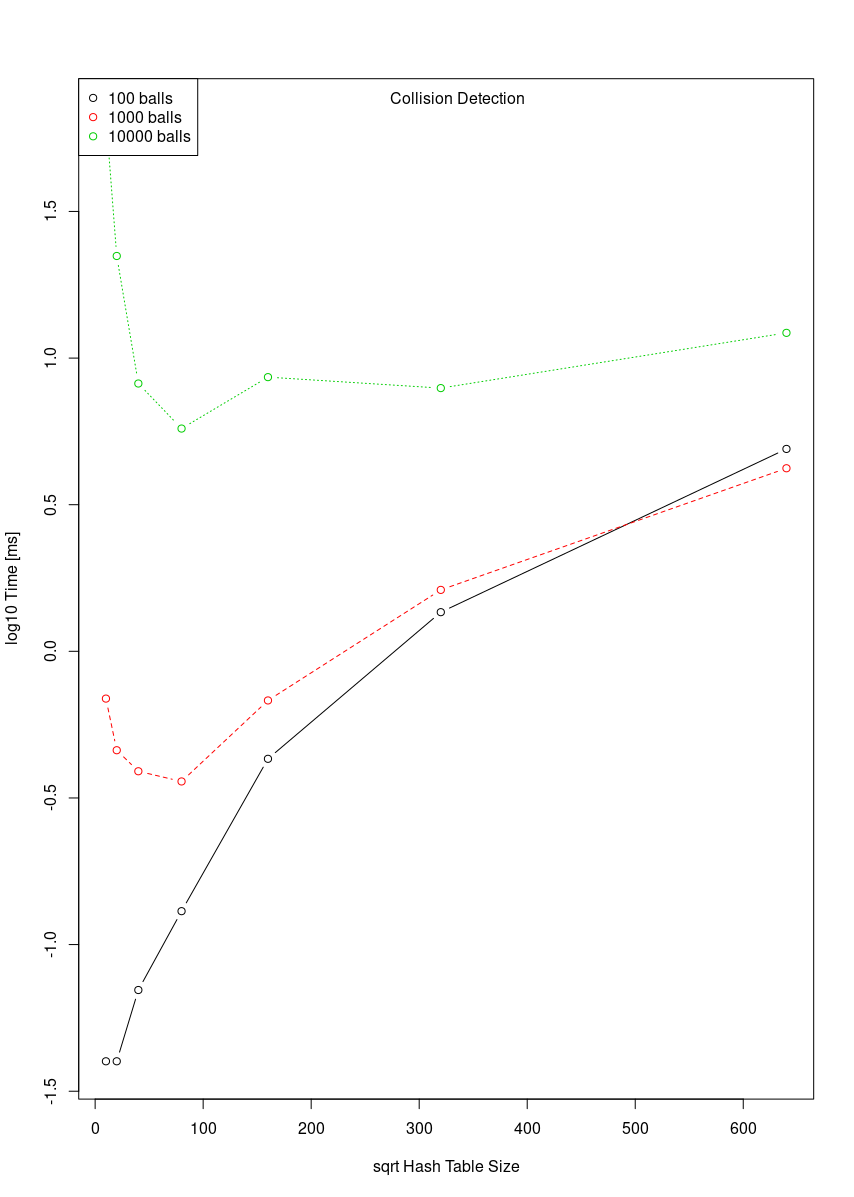
\includegraphics[width=\linewidth]{resources/collision_detection.png}
\end{figure}

\FloatBarrier

\end{document}
